\section{Conceitos iniciais e sistemas de numeração}

\frame{
	\frametitle{Analógico x digital}
	\centering
	\scalebox{1.3}{
	

\tikzset{every picture/.style={line width=0.75pt}} %set default line width to 0.75pt        

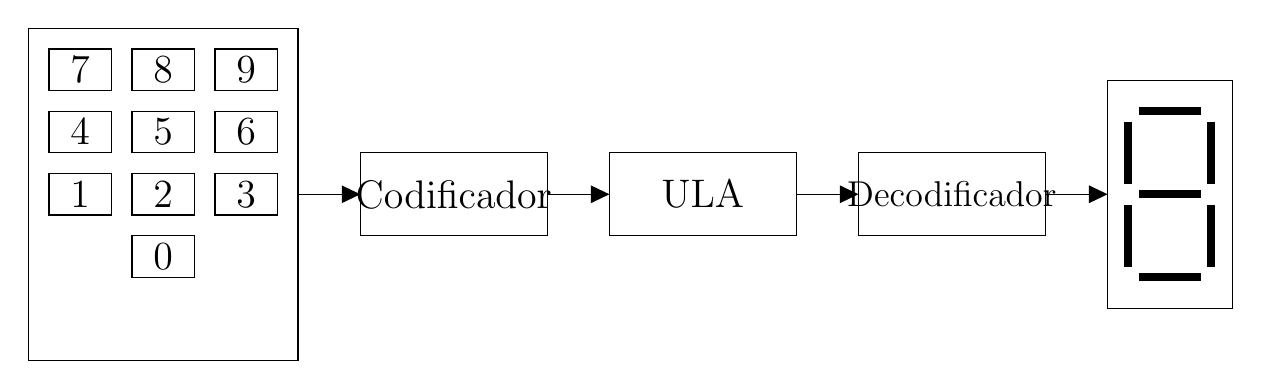
\begin{tikzpicture}[x=0.75pt,y=0.75pt,yscale=-1,xscale=1]
%uncomment if require: \path (0,300); %set diagram left start at 0, and has height of 300

%Shape: Rectangle [id:dp8798188650405219] 
\draw   (30,50) -- (160,50) -- (160,210) -- (30,210) -- cycle ;
%Shape: Rectangle [id:dp593444354888008] 
\draw   (40,60) -- (70,60) -- (70,80) -- (40,80) -- cycle ;
%Shape: Rectangle [id:dp4412846627526852] 
\draw   (80,60) -- (110,60) -- (110,80) -- (80,80) -- cycle ;
%Shape: Rectangle [id:dp2343273962035186] 
\draw   (120,60) -- (150,60) -- (150,80) -- (120,80) -- cycle ;
%Shape: Rectangle [id:dp05777918912875246] 
\draw   (40,90) -- (70,90) -- (70,110) -- (40,110) -- cycle ;
%Shape: Rectangle [id:dp9955010424516375] 
\draw   (80,90) -- (110,90) -- (110,110) -- (80,110) -- cycle ;
%Shape: Rectangle [id:dp24021539717259266] 
\draw   (120,90) -- (150,90) -- (150,110) -- (120,110) -- cycle ;
%Shape: Rectangle [id:dp36169684584711925] 
\draw   (40,120) -- (70,120) -- (70,140) -- (40,140) -- cycle ;
%Shape: Rectangle [id:dp7232437677097003] 
\draw   (80,120) -- (110,120) -- (110,140) -- (80,140) -- cycle ;
%Shape: Rectangle [id:dp6884539525496838] 
\draw   (120,120) -- (150,120) -- (150,140) -- (120,140) -- cycle ;
%Shape: Rectangle [id:dp9961423077173726] 
\draw   (80,150) -- (110,150) -- (110,170) -- (80,170) -- cycle ;
%Shape: Rectangle [id:dp6643057105712631] 
\draw   (190,110) -- (280,110) -- (280,150) -- (190,150) -- cycle ;
%Shape: Rectangle [id:dp7094011053258715] 
\draw   (550,75) -- (610,75) -- (610,185) -- (550,185) -- cycle ;
%Shape: Rectangle [id:dp2693438921699036] 
\draw   (310,110) -- (400,110) -- (400,150) -- (310,150) -- cycle ;
%Shape: Rectangle [id:dp3654960401722005] 
\draw   (430,110) -- (520,110) -- (520,150) -- (430,150) -- cycle ;
%Straight Lines [id:da6667328032348829] 
\draw    (160,130) -- (188,130) ;
\draw [shift={(190,130)}, rotate = 180] [fill={rgb, 255:red, 0; green, 0; blue, 0 }  ][line width=0.75]  [draw opacity=0] (8.93,-4.29) -- (0,0) -- (8.93,4.29) -- cycle    ;

%Straight Lines [id:da5165651690517046] 
\draw    (280,130) -- (308,130) ;
\draw [shift={(310,130)}, rotate = 180] [fill={rgb, 255:red, 0; green, 0; blue, 0 }  ][line width=0.75]  [draw opacity=0] (8.93,-4.29) -- (0,0) -- (8.93,4.29) -- cycle    ;

%Straight Lines [id:da17751850693095572] 
\draw    (400,130) -- (428,130) ;
\draw [shift={(430,130)}, rotate = 180] [fill={rgb, 255:red, 0; green, 0; blue, 0 }  ][line width=0.75]  [draw opacity=0] (8.93,-4.29) -- (0,0) -- (8.93,4.29) -- cycle    ;

%Straight Lines [id:da4998570413390182] 
\draw [color={rgb, 255:red, 0; green, 0; blue, 0 }  ,draw opacity=1 ][line width=3]    (560,95) -- (560,125) ;


%Straight Lines [id:da05287212083080073] 
\draw [color={rgb, 255:red, 0; green, 0; blue, 0 }  ,draw opacity=1 ][line width=3]    (600,95) -- (600,125) ;


%Straight Lines [id:da9146969001147236] 
\draw [color={rgb, 255:red, 0; green, 0; blue, 0 }  ,draw opacity=1 ][line width=3]    (560,135) -- (560,165) ;


%Straight Lines [id:da37610179690179124] 
\draw [color={rgb, 255:red, 0; green, 0; blue, 0 }  ,draw opacity=1 ][line width=3]    (600,135) -- (600,165) ;


%Straight Lines [id:da2798262228013664] 
\draw [color={rgb, 255:red, 0; green, 0; blue, 0 }  ,draw opacity=1 ][line width=3]    (595,130) -- (565,130) ;


%Straight Lines [id:da15184615547446478] 
\draw [color={rgb, 255:red, 0; green, 0; blue, 0 }  ,draw opacity=1 ][line width=3]    (595,90) -- (565,90) ;


%Straight Lines [id:da20609816632014244] 
\draw [color={rgb, 255:red, 0; green, 0; blue, 0 }  ,draw opacity=1 ][line width=3]    (595,170) -- (565,170) ;


%Straight Lines [id:da16937059284664002] 
\draw    (520,130) -- (548,130) ;
\draw [shift={(550,130)}, rotate = 180] [fill={rgb, 255:red, 0; green, 0; blue, 0 }  ][line width=0.75]  [draw opacity=0] (8.93,-4.29) -- (0,0) -- (8.93,4.29) -- cycle    ;


% Text Node
\draw (135,70) node   {\Large $9$};
% Text Node
\draw (95,70) node   {\Large $8$};
% Text Node
\draw (55,70) node   {\Large $7$};
% Text Node
\draw (135,100) node   {\Large $6$};
% Text Node
\draw (135,130) node   {\Large $3$};
% Text Node
\draw (95,160) node   {\Large $0$};
% Text Node
\draw (95,130) node   {\Large $2$};
% Text Node
\draw (95,100) node   {\Large $5$};
% Text Node
\draw (55,100) node   {\Large $4$};
% Text Node
\draw (55,130) node   {\Large $1$};
% Text Node
\draw (235,130) node  [align=left] {\Large Codificador};
% Text Node
\draw (355,130) node  [align=left] {\Large ULA};
% Text Node
\draw (475,130) node [scale=0.9] [align=left] {\Large Decodificador};


\end{tikzpicture}
}
%	\centerline{\includegraphics[width=0.7\linewidth]{Figuras/Ch1/analogdig.png}}
}

\frame{
	\frametitle{Analógico x digital}
	\centering
	\scalebox{0.8}{
		\deftkzbds
	
\begin{tikzpicture}[auto, node distance=2cm,>=Latex]
	
	\node [input, name=input] {};
	
	\node [coordinate, right=of input] (junction) {};
	\draw (input) -- node[near start] {$E(z)$} (junction);
	
	\node [block, right=of junction] (ei) {$ C_i(z) $};
	\node [block, above=of ei] (kp) {$ C_p(z) $};
	\node [block, below=of ei] (cd) {$ C_d(z) $};
	
	\draw [->] (junction) -- (ei);
	\draw [->] (junction) |- (kp);
	\draw [->] (junction) |- (cd);
	
	\node [sum, right=2cm of ei] (sum) {$ \phantom{\sum} $};
	\draw (sum) ++(-8pt,-8pt) -- ++(16pt,16pt) ++(-16pt,0pt) -- +(16pt,-16pt);
	
	\draw [<-] (sum) -- node[very near start, above] {$ + $} (ei);
	\draw [<-] (sum) |- node[very near start, right] {$ + $} (kp);
	\draw [<-] (sum) |- node[very near start, left] {$ + $} (cd);
	
	\node [output, right=of sum] (output) {};
	\draw [->] (sum) -- node[near end] {$ U(z) $} (output);
\end{tikzpicture}}
%	\centerline{\includegraphics[width=0.8\linewidth]{Figuras/Ch1/rampaescada.png}}
}

\frame{
	\frametitle{Analógico x digital}
	\centerline{\includegraphics[width=0.7\linewidth]{Figuras/Ch1/multimetro.jpg}}
}

\frame{
	\frametitle{Vantagens e desvantagens}
	\begin{block}{Vantagens}
		\begin{itemize}
			\item Sistemas digitais são mais simples de serem projetados. 
			\item Maior facilidade em manter precisão e exatidão. 
			\item Operações podem ser programadas. 
			\item Menos afetados por ruídos.
			\item CI’s (Circuitos Integrados) podem ser fabricados com mais dispositivos.
		\end{itemize}
	\end{block}
}

\frame{
	\frametitle{Vantagens e desvantagens}
	\begin{block}{Desvantagens}
		\begin{itemize}
			\item O mundo é quase todo analógico. 
			\item Processar sinais digitais demanda tempo.
		\end{itemize}
	\end{block}
}

\frame{
	\frametitle{E no mundo real?}
	\begin{block}{Importante}
		Como converter?
	\end{block}

	\vspace{0.5cm}
	
	\centerline{\includegraphics[width=0.8\linewidth]{Figuras/Ch1/mundoreal.png}}
}

\frame{
	\frametitle{Sistemas de numeração}
	\begin{block}{As quatro bases numéricas}
		\begin{itemize}
			\item Decimal
			\item Binário
			\item Octal
			\item Hexadecimal
		\end{itemize}
	\end{block}
}

\frame{
	\frametitle{Sistemas de numeração}
	\begin{block}{Sistema decimal}
		\begin{itemize}
			\item Caracteres 0 a 9.
			\item Notação posicional -- base 10.
			\item MSB x LSB.
			\item Exemplos de representação.
		\end{itemize}
	\end{block}

	\vspace{0.3cm}
	\centerline{\includegraphics[width=0.5\linewidth]{Figuras/Ch1/decimal.jpg}}
}

\frame{
	\frametitle{Sistemas de numeração}
	\begin{block}{Sistema binário}
		\begin{itemize}
			\item 2 dígitos.
			\item Notação posicional -- base 2.
			\item MSB x LSB.
			\item Quantidade de dígitos para representar -- como?.
		\end{itemize}
	\end{block}

	\vspace{0.3cm}
	
	\centerline{\includegraphics[width=0.4\linewidth]{Figuras/Ch1/binario.jpg}}
}

\frame{
	\frametitle{Sistemas de numeração}
\begin{block}{Tipos de dados binários}
%	\renewcommand{\arraystretch}{1.2}
	\centering
	\resizebox{\textwidth}{!}{
		\begin{tabular}{p{8em}C{8em}}
			\toprule
			\thead{\normalsize Tipo de dado} & \text{\thead{\normalsize Tamanho \\ 
				\normalsize (em bits)}} \\ \midrule
			bit & 1 \\
			nibble & 4 \\
			byte & 8 \\
			word & 16 \\
			double word & 32 \\
			\bottomrule
		\end{tabular}
	}
	\end{block}
}

\frame{
	\frametitle{Aritmética binária}
	\begin{block}{Adição}
			
		\begin{equation*}
		\mathlarger{\mathlarger{\mathlarger{
			\begin{array}{@{}B1}
				00\carry 11 \\
				{} + 0101 \\ \hline
				0110 \\
			\end{array}}}}
		\end{equation*}
	\end{block}
}

\frame{
	\frametitle{Aritmética binária}
	\begin{block}{Subtração}
		
		\begin{equation*}
		\mathlarger{\mathlarger{\mathlarger{
					\begin{array}{@{}B2}
						1\tikzmark{p1} & \carry1\tikzmark{p2}\carry 011 \\
					{}-	0 	& 1101 \\ \hline
						0 	& 1110 \\
					\end{array}}}}
		\end{equation*}
		
		\begin{tikzpicture}[overlay,remember picture]
			\draw (p1) ++(6,5.1) -- +(0.2,0.5);
			\draw (p1) ++(6.35,5.1) -- +(0.2,0.5);
		\end{tikzpicture}
	\end{block}
}

\frame{
	\frametitle{Aritmética binária}
	\begin{block}{Multiplicação}
		\centering
		\binmult{5}{6}
	\end{block}
%		\centerline{\includegraphics[width=0.5\linewidth]{Figuras/Ch1/multbin.png}}
}


\section*{Conversão entre bases numéricas}

\frame{
	\frametitle{Conversão binário-decimal}
	\begin{block}{Procedimento}
		\begin{itemize}
			\item Se dá pela soma das multiplicações de cada termo por sua potência de base 2 equivalente.
		\end{itemize}
	
		\centering
		\ConvertFromBase{2}{11001}
	\end{block}
%	\centerline{\includegraphics[width=0.5\linewidth]{Figuras/Ch1/bindec.png}}
}

\frame{
	\frametitle{Conversão decimal-binário}
	\begin{block}{Procedimento}
		\begin{itemize}
			\item Método das divisões sucessivas 
		\end{itemize}
	
		\vspace{0.5cm}
	
		\centering
		\begin{tabular}{c}
			\basetenconversiontable{12}{2}
		\end{tabular}
	\end{block}
%	\centerline{\includegraphics[width=0.5\linewidth]{Figuras/Ch1/decbin.png}}
}

\frame{
	\frametitle{Conversão fração decimal-binário}
	\begin{block}{Procedimento}
		\begin{itemize}
			\item Método das multiplicações sucessivas
		\end{itemize}
	
		\vspace{0.5cm}
		
		\ConvertitEnBaseB{3.75}{2}
	\end{block}
}

\section*{Exercícios}

\frame{
	\frametitle{Exercícios}

	\begin{block}{}
		01. Converter os seguintes números binários para decimais:

		\begin{itemize}
			\item \num{11111}$ _2 $
			\item \num{1001100}$ _2 $
			\item \num{1011,11}$ _2 $
			\item \num{1100,0011}$ _2 $
		\end{itemize}

		02. Converter os seguintes números decimais para binários:

		\begin{itemize}
			\item \num{215}
			\item \num{102}
			\item \num{9,92}
			\item \num{7,47}
		\end{itemize}
	\end{block}
}

\section*{Referências}

\frame{
	\frametitle{Referências e exercícios complementares}
	\begin{itemize}
		\item IDOETA, Ivan V. e CAPUANO, Francisco G. Elementos de Eletrônica Digital. São Paulo: Editora Érica, ed. 40. 2008.
	\end{itemize}

	\centering{\alert{Página 36 - \textbf{1.6.1 até 1.6.5, 1.6.17 até 1.6.19}}}
}